
\chapter{Manual de usuario}
\label{cha:manual-usuario}

\section{Introducción}
\label{sec:intro-manual-de-usuario}

Este apéndice se va a dividir en dos secciones diferenciadas donde se va a explicar como instalar y configurar todas las herramientas necesarias para la puesta a punto del proyecto. Y por otro lado, un manual de usuario donde se va a explicar como ejecutar cada uno de los algoritmos que se han utilizado en los capítulos \ref{cha:desarrollo} y \ref{cha:resultados}.
Cabe destacar que, tal y como se indica en el sección \ref{sec:intro-pliego}, el equipo donde se instalará todo el software descrito en este apartado para programar los distintos algoritmos, tiene un sistema operativo Ubuntu 18.04.4 LTS. Por tanto, todos los comandos de instalaciones y puesta en funcionamiento estarán orientados a un equipo que disponga de Linux.

\section{Guía de instalación}
\label{sec:sec-guia-instalacion}

\subsection{Instalación de Git}
\label{subsec:instalacion-git}

Git es una herramienta de control de versiones distribuido de código que trabaja de una manera muy rápida y potente. Tiene un sistema para trabajar mediante ramas que pueden seguir una línea de progreso diferente a la principal, de tal manera que se pueden hacer pruebas del código o que distintas personas trabajen en ramas paralelas y posteriormente, en una versión final de la implementación, se pueda incluir en la rama principal. Para proyectos como el presente, es necesario tener disponible historial completo de versiones para su correcto desarrollo.

Para poder instalar Git abra el terminal y ejecute los siguientes comandos:

\vspace{0.5cm}
\begin{lstlisting}[language=iPython,caption=Instalación de Git,captionpos=b,label={lst:install-git}]
# Actualizar paquetes de los repositorios
sudo apt-get update

# Instalacion de Git con todas sus depedencias
sudo apt-get install git-all
\end{lstlisting}

\subsection{Instalación de Anaconda}
\label{subsec:instalacion-anaconda}

Anaconda se trata de la \textit{suite} más compleja para la Ciencia de Datos en R y Python, lenguajes de programación que actualmente son líderes en Machine Learning, Inteligencia Artificial y Big Data. Esta \textit{suite} gratuita y multiplataforma dispone de las \gls{ide}'s y librerías adecuadas para su manejo. Con Anaconda se evita tener que instalar manualmente un \gls{ide} y el lenguaje Python, con sus correspondientes librerías, que en ocasiones puede ser una operación tediosa y compleja.

\begin{enumerate}
    \item Accede al siguiente enlace \cite{inst-conda} disponible en la bibliografía y descargue la versión más reciente del instalador de Anaconda para Linux:
    
    \begin{figure}[ht]
    \centering
    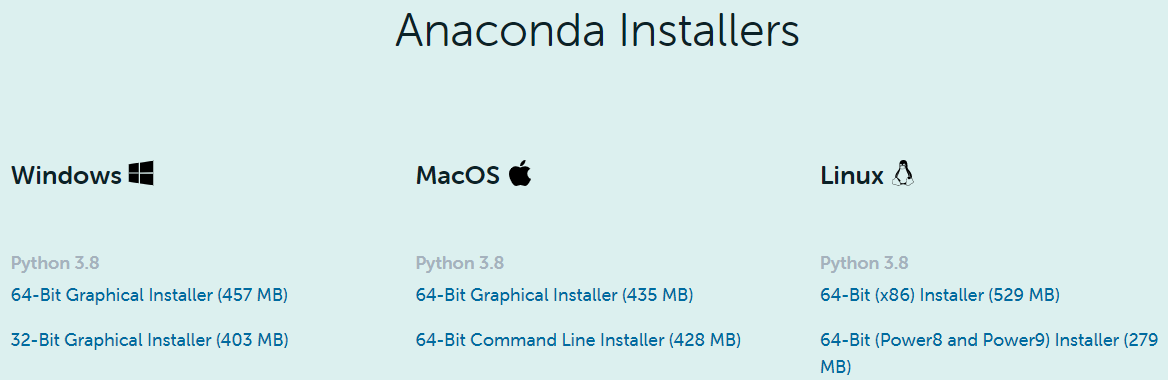
\includegraphics[width=0.8\textwidth]{img/appendix/C/anaconda-installer.png}
    \caption{\label{fig:anaconda-download}Descarga del instalador de Anaconda}
    \end{figure}

    \item Abra el terminal y acceda a la carpeta \texttt{Downloads} donde ha descargado el instalador. Es recomendable verificar la integridad del instalador mediante la suma de comprobación SHA-256:
    
    \vspace{0.5cm}
    
    % Los siguientes \begin{lstlisting}[... no están tabulados porque si no se crea una linea adicional de en las celdas
    % además de que saldría todo el código tabulado dentro de las celdas y no queda bien
    
\begin{lstlisting}[language=iPython,caption=Verificación de la integridad de la instalación de Anaconda,captionpos=b,label={lst:verificar-sha256}]
# Acceder a la carpeta Downloads del usuario
cd /home/<username>/Downloads

# Verificacion de la integridad del instalador
sha256sum Anaconda3-2020.02-Linux-x86_64.sh
\end{lstlisting}
    
    \item Ejecute la secuencias de comandos de Anaconda. Presione \texttt{yes} para aceptar los términos de la licencia. Pulse a continuación \texttt{ENTER} cuando seleccione la ubicación de la instalación y finalmente presione \texttt{yes} para confirmar el \texttt{PATH} de Anaconda con tu \texttt{.bashrc}:
    
    \vspace{0.5cm}
    
\begin{lstlisting}[language=iPython,caption=Ejecutar el instalador de Anaconda para Linux,captionpos=b,label={lst:install-conda}]
# Ejecutar el instalador de Anaconda para Linux
bash Anaconda3-2020.02-Linux-x86_64.sh
\end{lstlisting}
    
    \item Cuando se complete la instalación cierre y abra el terminal de nuevo, o bien ejecute el siguiente comando:
    
    \vspace{0.5cm}
    
\begin{lstlisting}[language=iPython,caption=Hacer efectivo los cambios en el fichero .bashrc,captionpos=b,label={lst:source-bashrc}]
# Hacer efectivos los cambios realizados en .bashrc
source /home/<username>/.bashrc
\end{lstlisting}
\end{enumerate}

\subsection{Descarga de los repositorios del proyecto}
\label{subsec:descargas-repos}

En esta sección se indica como descargar los repositorios de GitHub donde se han programado los algoritmos de detección y seguimiento de objetos abandonados. Para ello, se debe de ejecutar los comandos que se muestran a continuación:

\vspace{0.5cm}

\begin{lstlisting}[language=iPython,caption=Descarga repositorio,captionpos=b,label={lst:descarga-repo}]
# Acceder a la carpeta Documents del usuario
cd /home/<username>/Documents

# Clonar los dos repositorios de GitHub
git clone https://github.com/jmudy/tensorflow-yolov4-tflite
git clone https://github.com/jmudy/yolov4-deepsort.git

# Acceder al repositorio de deteccion de objetos con YOLOv4
cd tensorflow-yolov4-tflite

# O bien al de seguimiento y deteccion de objetos abandonados con YOLOv4 y Deep SORT
cd yolov4-deepsort
\end{lstlisting}

\subsection{Crear entorno virtual con Anaconda}
\label{subsec:creacion-entorno}

Con la finalidad de evitar la tediosa y larga instalación de \gls{cuda} y \gls{cudnn} y tener únicamente instaladas las librerías necesarias para que funcione el código, se va a instalar un entorno virtual en Anaconda.

Desde cualquiera de las carpetas de los repositorios de Github que se han clonado, hay dos ficheros con extensión .yml, donde viene indicadas la versión de Python que se va a necesitar, la versión de \gls{cuda} y \gls{cudnn} así como las librerías y dependencias necesarias. Para utilizar \gls{cuda} es necesario disponer de una \gls{gpu} de NVIDIA. Es muy importante verificar la capacidad de cálculo de la tarjeta gráfica NVIDIA que se emplee. En la siguiente dirección \cite{cuda-gpus} se puede comprobar la capacidad de cálculo de los distintos modelos o bien puede consultar la que esté utilizando introduciendo los siguientes comandos en el terminal:

\begin{lstlisting}[language=iPython,caption=Comprobar capacidad computación de la GPU,captionpos=b,label={lst:check-compute-capability}]
# Iniciar Python en terminal
python

# Importar libreria tensorflow
import tensorflow as tf

# Test sobre el dispositivo GPU que se este empleando
tf.test.gpu_device_name()
\end{lstlisting}

La capacidad de cálculo mínima para poder utilizar \gls{cuda} junto a la librería tensorflow-gpu es de 3.5. En función de la \gls{gpu} que se disponga, ejecute uno de los siguientes comandos para crear un entorno virtual de Anaconda con Python 3.7.0:

\vspace{0.5cm}

\begin{lstlisting}[language=iPython,caption=Creación entorno virtual en Anaconda,captionpos=b,label={lst:crear-env}]
# Si tu GPU tiene una capacidad de calculo < 3.5
conda env create -f conda-cpu.yml

# Si tu GPU tiene una capacidad de calculo >= a 3.5
conda env create -f conda-gpu.yml
\end{lstlisting}

Una vez instalado el entorno virtual se puede activar ejecutando el siguiente comando:

\vspace{0.5cm}

\begin{lstlisting}[language=iPython,caption=Activar entorno virtual de Anaconda,captionpos=b,label={lst:activar-env}]
# Si instalaste el entorno con conda-cpu.yml
conda activate yolov4-cpu

# Si instalaste el entorno con conda-gpu.yml
conda activate yolov4-gpu
\end{lstlisting}

\subsection{Descargar los datasets}
\label{subsec:descarga-datasets}

Los enlaces para descargar los datasets que se han utilizado para evaluar los distintos algoritmos a lo largo del proyecto se encuentran a continuación:

\begin{itemize}
    \item \gls{pets} dataset \url{http://www.cvg.reading.ac.uk/PETS2007/data.html} \cite{pets2007-dataset}
    \item \gls{avss} dataset \url{http://www.eecs.qmul.ac.uk/~andrea/avss2007_d.html} \cite{AVSSAB2007-dataset}
    \item \gls{gba2018} dataset \url{https://bit.ly/3tIJdUx} \cite{gba-dataset}
    \item \gls{aboda} dataset \url{https://github.com/kevinlin311tw/ABODA} \cite{aboda-dataset}
    \item \gls{coco} dataset \url{https://cocodataset.org/#download} \cite{lin2015microsoft}
    \item \gls{oidv4} dataset \url{https://storage.googleapis.com/openimages/web/index.html} \cite{Kuznetsova_2020}
    
\end{itemize}

\section{Guía de ejecución}
\label{sec:guia-ejecucion}

En esta parte se especifica los comandos que se deben ejecutar para poner en funcionamiento el algoritmo de detección de objetos, el algoritmo de seguimiento de personas y objetos y por último, el algoritmo de detección de objetos abandonados. Cabe destacar que el repositorio con nombre \texttt{yolov4-deepsort} se utiliza tanto para ejecutar el script de seguimiento con \gls{deepsort} como para ejecutar el algoritmo de detección de objetos abandonados.

\subsection{Ejecutar algoritmo de detección de objetos YOLOv4}
\label{subsec:ejecutar-deteccion-yolov4}

Para ejecutar el algoritmo de detección de \gls{yolov4} en el framework Tensorflow entre en la carpeta del repositorio \texttt{tensorflow-yolov4-tflite}, descargue y convierta el modelo Darknet a Tensorflow. Para ello, abra el terminal y ejecute los siguientes comandos:

\vspace{0.5cm}
\begin{lstlisting}[language=iPython,caption=Descarga de pesos y conversion modelo YOLOv4,captionpos=b,label={lst:descarga-weights-convertir-modelo}]
# Descargar los pesos de YOLOv4
wget https://github.com/AlexeyAB/darknet/releases/download/darknet_yolo_v3_optimal/yolov4.weights -P ./data/

# Convertir modelo Darknet de YOLOv4 a modelo Tensorflow
python save_model.py --weights ./data/yolov4.weights --output ./checkpoints/yolov4-608 --input_size 608 --model yolov4
\end{lstlisting}

Por último, introduzca el vídeo que se quiera analizar dentro de la carpeta del repositorio. Se recomienda introducir los vídeos a analizar en la carpeta \texttt{./data/video/} y los vídeos generados en la carpeta \texttt{./detections}.

\vspace{0.5cm}
\begin{lstlisting}[language=iPython,caption=Ejecutar script detección de objetos con YOLOv4 en Tensorflow,captionpos=b,label={lst:ejecutar-yolov4-tf}]
# Cambiar la ruta donde se encuentre el video que se quiera analizar y la ruta donde se
# quiere guardar el video que se genere
python detect_video.py --weights ./checkpoints/yolov4-608 --size 608 --model yolov4 --video <path_to_input_video> --output <path_to_output_video>
\end{lstlisting}

Si no se dispone del equipo necesario para instalar todas las dependencias necesarias se recomienda acceder al siguiente \href{https://colab.research.google.com/drive/1ZwcfV2hFZKcsyXaqKp9AGuEi5TY-QwVW?usp=sharing}{link} donde se facilita un Notebook de Google Colab para ejecutar exactamente los mismos comandos desde el servicio cloud de Google.

Recuerde que, tal y como se explicó en la sección \ref{sec:desarrollo-yolov4}, también se pueden modificar parámetros como el tamaño del resize, el umbral del \gls{iou} o el umbral de confianza añadiendo los flags que sean pertinentes.

\subsection{Ejecutar algoritmo de seguimiento de objetos YOLOv4 + Deep SORT}
\label{subsec:ejecutar-seguimiento-yolov4-deepsort}

Para ejecutar el algoritmo de seguimiento con \gls{deepsort} y \gls{yolov4} entre en la carpeta del repositorio \texttt{yolov4-deepsort}, descargue y convierta el modelo Darknet a Tensorflow de igual manera que se hizo el script \ref{lst:descarga-weights-convertir-modelo} de la sección \ref{subsec:ejecutar-deteccion-yolov4}.

Una vez se tenga el modelo de YOLOv4 convertido, introduzca el vídeo que se quiera analizar dentro de la carpeta del repositorio. Se recomienda introducir los vídeos a analizar en la carpeta \texttt{./data/video/} y los vídeos generados en la carpeta \texttt{./outputs}.

Por último, ejecutar el script de seguimiento de personas y objetos introduciendo el siguiente comando en el terminal:

\vspace{0.5cm}
\begin{lstlisting}[language=iPython,caption=Ejecutar script seguimiento de personas y objetos con DeepSORT,captionpos=b,label={lst:ejecutar-yolov4-deepsort}]
# Cambiar la ruta donde se encuentre el video que se quiera analizar y la ruta donde se
# quiere guardar el video que se genere
python detect_video.py --weights ./checkpoints/yolov4-608 --size 608 --model yolov4 --video <path_to_input_video> --output <path_to_output_video>
\end{lstlisting}

Si no se dispone del equipo necesario para instalar todas las dependencias necesarias se recomienda acceder al siguiente \href{https://colab.research.google.com/drive/18vL9LH8e9VaimA9LzBD35Cn4AOm6C17I?usp=sharing}{link} donde se facilita un Notebook de Google Colab para ejecutar exactamente los mismos comandos desde el servicio cloud de Google.

Recuerde que, tal y como se explicó en la sección \ref{sec:desarrollo-yolov4}, también se pueden modificar parámetros como el tamaño del resize, el umbral del \gls{iou} o el umbral de confianza añadiendo los flags que sean pertinentes.

\subsection{Ejecutar algoritmo de detección de objetos abandonados}
\label{subsec:ejecutar-deteccion-abandoned-object}

Para ejecutar el algoritmo de detección de objetos abandonados con \gls{deepsort} y \gls{yolov4} entre en la carpeta del repositorio \texttt{yolov4-deepsort}, descargue y convierta el modelo Darknet a Tensorflow de igual manera que se hizo el script \ref{lst:descarga-weights-convertir-modelo} de la sección \ref{subsec:ejecutar-deteccion-yolov4}.

Una vez se tenga el modelo de YOLOv4 convertido, introduzca el vídeo que se quiera analizar dentro de la carpeta del repositorio. Se recomienda introducir los vídeos a analizar en la carpeta \texttt{./data/video/} y los vídeos generados en la carpeta \texttt{./outputs}.

Por último, ejecutar el script de detección de objetos abandonados introduciendo el siguiente comando en el terminal:

\vspace{0.5cm}
\begin{lstlisting}[language=iPython,caption=Ejecutar script detección de objetos abandonados con YOLOv4 y Deep SORT,captionpos=b,label={lst:ejecutar-yolov4-abandoned-object}]
# Cambiar la ruta donde se encuentre el video que se quiera analizar y la ruta donde se
# quiere guardar el video que se genere
python abandoned_object.py --weights ./checkpoints/yolov4-608 --size 608 --model yolov4 --video <path_to_input_video> --output <path_to_output_video>
\end{lstlisting}

Si no se dispone del equipo necesario para instalar todas las dependencias necesarias se recomienda acceder al siguiente \href{https://colab.research.google.com/drive/18vL9LH8e9VaimA9LzBD35Cn4AOm6C17I?usp=sharing}{link} donde se facilita un Notebook de Google Colab para ejecutar exactamente los mismos comandos desde el servicio cloud de Google.

Recuerde que, tal y como se explicó en la sección \ref{sec:desarrollo-yolov4}, también se pueden modificar parámetros como el tamaño del resize, el umbral del \gls{iou} o el umbral de confianza añadiendo los flags que sean pertinentes.